\chapter{हृदय और हृद्-चक्र}\label{ch:b2:heart}

किसी मेंढक का \omterm{def:b2:heart:anatomy}{हृदय} काटकर निकालिए और उसे लवण-विलयन में डाल दीजिए, और वह
घंटों धड़कता रहता है --- कोई तंत्रिका नहीं, कोई मस्तिष्क नहीं, कोई \omterm{def:b2:blood-circulation:blood}{रक्त}
नहीं, बस एक पेशी जो लगभग हर सेकंड अपने आप सिकुड़ती है क्योंकि उसकी
कोशिकाओं का एक छोटा-सा टुकड़ा चुप नहीं बैठ सकता। कोई मानव \omterm{def:b2:heart:anatomy}{हृदय} यह
जीवन भर में कोई तीन अरब बार करता है, और कोई दो
करोड़ लीटर चलाता है, बिना कभी बंद हुए। यह
अध्याय उसी पंप के बारे में है: उसके कक्ष तथा कपाट, भरने और
ख़ाली होने का चक्र तथा वे दाब जो उसे चलाते हैं, वह विद्युत्
तंत्र जो उसका समय बाँधता है और वह चिह्न जो वह त्वचा पर छोड़ता है, वह नियम
जो उसे अपना निर्गम अपने अंतर्वाह से धड़कन-दर-धड़कन मिलाने देता है, और वे
तंत्रिकाएँ तथा हॉर्मोन जो उसकी चाल और बल समंजित करते हैं।

\section{वह पंप}

\begin{definition}[कक्ष और कपाट]\label{def:b2:heart:anatomy}
\index{हृदय}\index{अलिंद}\index{निलय}\index{हृद्-कपाट}
हृदय अगल-बग़ल दो पंप हैं, और हर एक में एक \emph{अलिंद} है जो
\omterm{def:b2:blood-circulation:vessels}{शिराओं} से \omterm{def:b2:blood-circulation:blood}{रक्त} लेता है और एक \emph{निलय} जो उसे किसी
\omterm{def:b2:blood-circulation:vessels}{धमनी} में निकालता है। दायाँ हृदय महाशिराओं से \omterm{def:b2:blood-circulation:blood}{रक्त} लेता है
और उसे फुफ्फुस \omterm{def:b2:blood-circulation:vessels}{धमनी} से होकर फेफड़ों को भेजता है; बायाँ
हृदय उसे फुफ्फुस \omterm{def:b2:blood-circulation:vessels}{शिराओं} से वापस लेता है और महाधमनी से होकर
देह भर घुमाता है। चार कपाट उस प्रवाह को एकतरफ़ा बनाते हैं:
\emph{अलिंद-निलय कपाट} (दाईं ओर त्रिवलनी, बाईं ओर
द्विवलनी), यानी ऐसे फलक जो रज्जुओं से पैपिलरी पेशियों से बँधे हैं ताकि
वे वापस अलिंद में उड़ा न दिए जाएँ; और
\emph{अर्धचंद्राकार कपाट} (फुफ्फुसीय तथा महाधमनीय), यानी तीन जेबें जो
धमनीय दाब के निलय से बढ़ते ही भरकर बंद हो जाती हैं।
वे कपाट निष्क्रिय हैं: वे केवल दाब-अंतरों पर खुलते और बंद
होते हैं। निलय-भित्ति \emph{हृद्पेशी} है, यानी
शाखित कोशिकाओं की रेखित पेशी जो सिरे-से-सिरे
\emph{अंतर्वेशित चकतियों} से जुड़ी हैं जिनमें गैप संधियाँ भरी हैं, इसलिए पूरा
निलय विद्युत् रूप से एक ही कोशिका है और एक की तरह सिकुड़ता है; बाएँ
निलय की भित्ति दाएँ से तीन गुना मोटी है क्योंकि वह
पाँच गुना दाब के विरुद्ध पंप करता है। हृद्-पेशी को उसकी अपनी
\emph{हृद्-धमनियाँ} पोसती हैं, जो अनुशिथिलन में भरती हैं, और वह
लगभग पूरी तरह वायवीय उपापचय पर चलती है --- वह उधार नहीं ले सकती।
\end{definition}

\begin{omfigure}
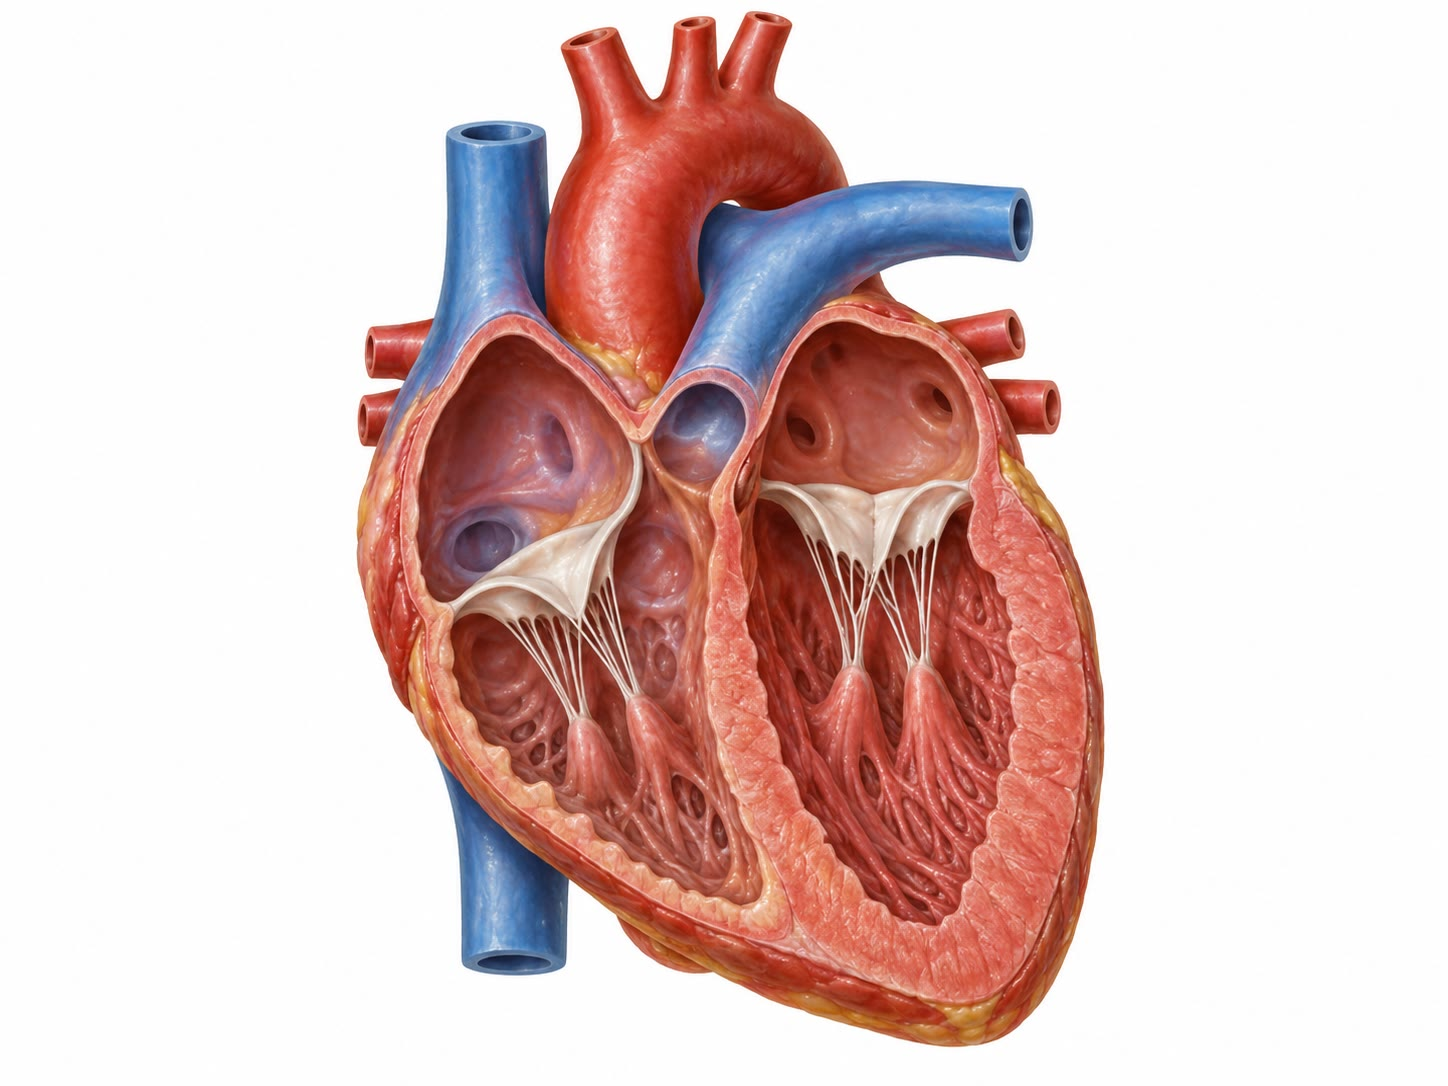
\includegraphics[width=0.55\linewidth]{images/book4/ai/b4-17-heart-cutaway.jpg}

{\small अग्र काट में \omterm{def:b2:heart:anatomy}{हृदय}: ऊपर दो \omterm{def:b2:heart:anatomy}{अलिंद}, नीचे दो \omterm{def:b2:heart:anatomy}{निलय},
मोटा बायाँ \omterm{def:b2:heart:anatomy}{निलय}, अपनी रज्जुओं समेत अलिंद-निलय कपाट,
और ऊपर से निकलती दो महावाहिकाएँ।}
\end{omfigure}

\begin{proposition}[हृद्-चक्र]\label{prop:b2:heart:cycle}
\index{हृद्-चक्र}\index{प्रकुंचन}\index{अनुशिथिलन}\index{आघात-आयतन}\index{निष्कासन अंश}
विश्राम में एक धड़कन लगभग \qty{0.8}{s} चलती है। \emph{अनुशिथिलन}
(\qty{0.5}{s}): \omterm{def:b2:heart:anatomy}{निलय} ढीले होते हैं, उनका दाब \omterm{def:b2:heart:anatomy}{अलिंदों} से
नीचे गिरता है, अलिंद-निलय कपाट खुलते हैं और \omterm{def:b2:blood-circulation:blood}{रक्त} भीतर बहता है,
अधिकतर निष्क्रिय रूप से, फिर अलिंद-संकुचन के एक अंतिम धक्के से;
वह \omterm{def:b2:heart:anatomy}{निलय} अनुशिथिलन के अंत में लगभग \qty{120}{mL} थामे होता है (यानी
\emph{अंत-अनुशिथिलनी आयतन})। \emph{प्रकुंचन} (\qty{0.3}{s}):
\omterm{def:b2:heart:anatomy}{निलय} सिकुड़ते हैं; उनका दाब अलिंदीय दाब से बढ़ते ही
अलिंद-निलय कपाट बंद हो जाते हैं (पहली हृद्-ध्वनि,
``लब''), और सेकंड के कुछ सौवें भाग तक वह \omterm{def:b2:heart:anatomy}{निलय}
किसी बंद कक्ष को भींचता है --- \emph{समआयतनी संकुचन} ---
जब तक उसका दाब धमनीय दाब को पार न कर ले (बाईं ओर \qty{80}{mmHg}),
और तब अर्धचंद्राकार कपाट खुलते हैं और \omterm{def:b2:blood-circulation:blood}{रक्त} निकाला जाता है। बायाँ
\omterm{def:b2:heart:anatomy}{निलय} \qty{120}{mmHg} तक पहुँचता है और लगभग
\qty{70}{mL} बाहर करता है (यानी \emph{\omterm{prop:b2:heart:cycle}{आघात-आयतन}}, यानी \qty{60}{\%}
का कोई \emph{\omterm{prop:b2:heart:cycle}{निष्कासन अंश}}); ज्यों ही वह ढीला होता है, उसका दाब
महाधमनी से नीचे गिरता है, महाधमनी-कपाट चटककर बंद होता है (दूसरी ध्वनि, ``डब''),
और कोई समआयतनी शिथिलन उस दाब को
अलिंदीय स्तर तक ले आता है, और तब भरना फिर शुरू होता है। दायाँ \omterm{def:b2:heart:anatomy}{हृदय} वही
पाँचवें भाग दाब पर करता है, और वही आयतन निकालता है।
\end{proposition}

\begin{omfigure}
\begin{tikzpicture}
\begin{axis}[
  width=0.9\linewidth, height=7.2cm,
  axis x line=bottom, axis y line=left,
  xmin=0, xmax=0.8, ymin=0, ymax=130,
  xlabel={चक्र में समय (s)}, ylabel={दाब (\unit{mmHg})},
  xlabel style={font=\small, at={(axis description cs:0.5,-0.1)}, anchor=north},
  ylabel style={font=\small},
  tick label style={font=\small}, xtick={0,0.1,0.3,0.8}, ytick={0,40,80,120},
  legend style={font=\scriptsize, at={(0.6,0.45)}, anchor=west, draw=none},
  clip=false,
]
% aortic pressure
\addplot[very thick, omThm] coordinates {(0,82) (0.05,80) (0.1,80) (0.12,95) (0.16,115) (0.2,120) (0.25,112) (0.3,100) (0.32,104) (0.34,100) (0.45,94) (0.6,88) (0.8,82)};
\addlegendentry{महाधमनी}
% left ventricular pressure
\addplot[very thick, omDef] coordinates {(0,5) (0.04,8) (0.05,10) (0.08,60) (0.1,80) (0.12,95) (0.16,115) (0.2,120) (0.25,112) (0.3,100) (0.32,60) (0.35,20) (0.38,5) (0.5,3) (0.7,5) (0.75,8) (0.8,5)};
\addlegendentry{बायाँ निलय}
% atrial pressure
\addplot[thick, omProp] coordinates {(0,6) (0.03,9) (0.06,6) (0.1,8) (0.15,6) (0.3,7) (0.36,10) (0.4,5) (0.6,6) (0.75,9) (0.8,6)};
\addlegendentry{बायाँ अलिंद}
\draw[dashed, gray] (axis cs:0.05,0) -- (axis cs:0.05,128); \node[font=\scriptsize, anchor=south, align=center] at (axis cs:0.05,128) {द्विवलनी\\बंद};
\draw[dashed, gray] (axis cs:0.1,0) -- (axis cs:0.1,128); \node[font=\scriptsize, anchor=south, align=center] at (axis cs:0.13,128) {महाधमनीय\\खुलता};
\draw[dashed, gray] (axis cs:0.31,0) -- (axis cs:0.31,128); \node[font=\scriptsize, anchor=south, align=center] at (axis cs:0.31,128) {महाधमनीय\\बंद};
\draw[dashed, gray] (axis cs:0.38,0) -- (axis cs:0.38,128); \node[font=\scriptsize, anchor=south, align=center] at (axis cs:0.4,128) {द्विवलनी\\खुलता};
\node[font=\scriptsize] at (axis cs:0.2,45) {प्रकुंचन};
\node[font=\scriptsize] at (axis cs:0.55,25) {अनुशिथिलन};
\end{axis}
\end{tikzpicture}

{\small एक धड़कन भर बाएँ \omterm{def:b2:heart:anatomy}{हृदय} में दाब। वह \omterm{def:b2:heart:anatomy}{निलय}
किसी बंद कक्ष को तब तक भींचता है जब तक वह महाधमनीय दाब से न बढ़ जाए,
जब तक वह उससे ऊपर है तब तक निकालता है, अलिंदीय दाब से नीचे गिरने तक
ढीला होता है, और भरता है।}
\end{omfigure}

\begin{theorem}[हृदय का काम]\label{thm:b2:heart:work}
\index{हृद्-कार्य}\index{दाब--आयतन पाश}
आयतन के सापेक्ष दाब के रूप में आलेखित करने पर बाएँ \omterm{def:b2:heart:anatomy}{निलय} की एक धड़कन
कोई पाश खींचती है --- नीचे-नीचे भरना, दाईं ओर ऊपर समआयतनी
संकुचन, ऊपर-ऊपर \qty{120}{mL} से \qty{50}{mL} तक निष्कासन,
बाईं ओर नीचे समआयतनी शिथिलन --- और उस पाश का
क्षेत्रफल उस धड़कन का यांत्रिक काम है:
\[
W = \oint P\,\mathrm{d}V \approx \bar P_{\text{निष्कासन}}\times \text{आघात-आयतन} \approx \qty{100}{mmHg}\times\qty{70}{mL} = \qty{0.93}{J}.
\]
मिनट भर में 72 धड़कनों पर बायाँ \omterm{def:b2:heart:anatomy}{निलय} लगभग \qty{1.1}{W} करता है, और
दायाँ \qty{0.2}{W}; \omterm{def:b2:heart:anatomy}{हृदय} का उपापचय कोई \qty{8}{W} है, इसलिए उसकी
यांत्रिक दक्षता \qty{15}{\%} के पास है, और बाक़ी ऊष्मा तथा
तनाव की लागत है। \omterm{def:b2:heart:anatomy}{हृदय} जिस दाब के विरुद्ध पंप करता है उसे चढ़ाना
(उच्च रक्तचाप, कोई सँकरा महाधमनी-कपाट) प्रति धड़कन काम उसी
अनुपात में चढ़ा देता है, और वह पेशी उत्तर में मोटी हो जाती है जैसे कोई भी पेशी होती है
--- जब तक उसकी हृद्-आपूर्ति उसके भार के साथ न चल सके।
\end{theorem}
\begin{proof}
काम बल गुणा दूरी है, और किसी चलती भित्ति पर काम करते किसी दाब के लिए,
दाब गुणा बहा गया आयतन: $\mathrm{d}W = P\,\mathrm{d}V$।
किसी बंद पाश भर शुद्ध काम घिरा हुआ क्षेत्रफल है (नीचे दाब पर
भरने में कम लगता है; ऊँचे दाब पर निष्कासन उससे कहीं अधिक
लौटाता है)। $\qty{100}{mmHg} = \qty{1.33e4}{Pa}$ और $\qty{70}{mL} =
\qty{7e-5}{m^3}$: $1.33\times 10^{4}\times 7\times 10^{-5} =
\qty{0.93}{J}$; गुणा प्रति सेकंड $1.2$ धड़कनें, \qty{1.1}{W}।
\end{proof}

\begin{omfigure}
\begin{tikzpicture}
\begin{axis}[
  width=0.62\linewidth, height=6cm,
  axis x line=bottom, axis y line=left,
  xmin=0, xmax=150, ymin=0, ymax=140,
  xlabel={बाएँ निलय का आयतन (\unit{mL})}, ylabel={दाब (\unit{mmHg})},
  xlabel style={font=\small, at={(axis description cs:0.5,-0.12)}, anchor=north},
  ylabel style={font=\small},
  tick label style={font=\small}, xtick={0,50,120}, ytick={0,80,120},
  clip=false,
]
\fill[omDef!12] (axis cs:50,5) -- (axis cs:120,8) -- (axis cs:120,80) -- (axis cs:110,115) -- (axis cs:80,122) -- (axis cs:50,100) -- cycle;
\draw[very thick, omDef, ->] (axis cs:50,5) -- (axis cs:120,8);
\draw[very thick, omDef, ->] (axis cs:120,8) -- (axis cs:120,80);
\draw[very thick, omDef, ->] (axis cs:120,80) .. controls (axis cs:110,118) and (axis cs:80,125) .. (axis cs:50,100);
\draw[very thick, omDef, ->] (axis cs:50,100) -- (axis cs:50,5);
\node[font=\scriptsize, anchor=south] at (axis cs:85,11) {भरना};
\node[font=\scriptsize, anchor=west] at (axis cs:122,44) {समआयतनी संकुचन};
\node[font=\scriptsize, anchor=south] at (axis cs:85,124) {निष्कासन};
\node[font=\scriptsize, anchor=east] at (axis cs:48,52) {शिथिलन};
\node[font=\scriptsize] at (axis cs:85,60) {क्षेत्रफल $=$ काम, \qty{0.9}{J}};
\end{axis}
\end{tikzpicture}

{\small बाएँ \omterm{def:b2:heart:anatomy}{निलय} का \omterm{thm:b2:heart:work}{दाब--आयतन पाश}। घिरा हुआ
क्षेत्रफल एक धड़कन का काम है; कोई ऊँचा धमनीय दाब उस पाश का
शीर्ष और उसके साथ वह काम चढ़ा देता है।}
\end{omfigure}

\section{हृदय की अपनी घड़ी}

\begin{proposition}[स्वचालिता और चालन]\label{prop:b2:heart:conduction}
\index{साइनु-अलिंद गाँठ}\index{गतिकारक}\index{अलिंद-निलय गाँठ}\index{पुर्किंजे तंतु}
वह धड़कन \emph{\omterm{prop:b2:heart:conduction}{साइनु-अलिंद गाँठ}} में उपजती है, यानी दाएँ
\omterm{def:b2:heart:anatomy}{अलिंद} की भित्ति में विशिष्ट पेशी-कोशिकाओं का एक टुकड़ा जिसका
झिल्ली-विभव कभी विश्राम नहीं करता: हर क्रिया-विभव के बाद वह
धीरे ऊपर सरकता है (कोई \emph{गतिकारक विभव}, जिसे कोई
सोडियम धारा चलाती है जो ऋण विभवों पर चालू होती है और कैल्सियम
वाहिकाएँ) जब तक वह देहली तक न पहुँचे और फिर न दगे, और यदि उसे छोड़ दिया जाए तो
मिनट भर में कोई सौ बार। वह आवेग
अलिंद-पेशी में, गैप संधियों से कोशिका-दर-कोशिका, फैलता है, और
\omterm{def:b2:heart:anatomy}{अलिंद} सिकुड़ते हैं; वह \emph{\omterm{prop:b2:heart:conduction}{अलिंद-निलय गाँठ}} तक पहुँचता है, यानी
\omterm{def:b2:heart:anatomy}{अलिंदों} और \omterm{def:b2:heart:anatomy}{निलयों} के बीच का एकमात्र विद्युत् सेतु, जो
धीरे चालन करती है और उसे सेकंड के दसवें भाग तक टालती है --- यानी \omterm{def:b2:heart:anatomy}{अलिंदों} को
\omterm{def:b2:heart:anatomy}{निलय} भरना पूरा करने भर का समय; फिर वह
\emph{हिस बंडल} और \emph{\omterm{prop:b2:heart:conduction}{पुर्किंजे तंतुओं}} से नीचे दौड़ता है, यानी तेज़ चालन वाली
ऐसी कोशिकाएँ जो उसे \qty{30}{ms} के भीतर पूरी निलय-पेशी तक
पहुँचा देती हैं, ताकि \omterm{def:b2:heart:anatomy}{निलय} शीर्ष से ऊपर की ओर,
एक इकाई की तरह, सिकुड़ें और \omterm{def:b2:blood-circulation:blood}{रक्त} को बहिर्वाह कपाटों की ओर चलाएँ। इस
तंत्र का हर भाग स्वयं गति दे सकता है, और हर एक पिछले से
धीरे (वह गाँठ 100 पर, \omterm{prop:b2:heart:conduction}{अलिंद-निलय गाँठ} 50 पर, \omterm{prop:b2:heart:conduction}{पुर्किंजे तंतु}
30 पर), ताकि यदि वह गाँठ चूक जाए तो कोई निचला केंद्र सँभाल ले --- किसी
धीमी दर पर।
\end{proposition}
\begin{proof}[प्रमाण-सामग्री]
कोई अलग किया हुआ \omterm{def:b2:heart:anatomy}{हृदय}, या साइनु-अलिंद ऊतक की कोई पट्टी, बिना तंत्रिकाओं के
किसी तश्तरी में धड़कती है; \omterm{def:b2:heart:anatomy}{निलय} की कोई पट्टी भी धड़कती है, पर अधिक धीरे।
केवल \omterm{prop:b2:heart:conduction}{साइनु-अलिंद गाँठ} को ठंडा या गरम करना पूरे
\omterm{def:b2:heart:anatomy}{हृदय} की दर बदल देता है; अलिंद-निलय बंडल काटना \omterm{def:b2:heart:anatomy}{निलयों} को अलग कर देता है,
जो तब अपनी ही धीमी लय पर धड़कते हैं जबकि \omterm{def:b2:heart:anatomy}{अलिंद}
उस गाँठ की पर चलते रहते हैं (हृद्-अवरोध)। किसी एक गाँठ-कोशिका से अभिलेख
वह धीमा अनुशिथिलनी विध्रुवण दिखाता है जो किसी साधारण पेशी-कोशिका
में नहीं है; उस गतिकारक धारा को रोकना उसे धीमा कर देता है।
\end{proof}

\begin{omfigure}
\begin{tikzpicture}[every node/.style={font=\scriptsize}, >=stealth]
  % simplified heart outline, scaled up
  \draw[thick, fill=omThm!6] (0,0) .. controls (-4.2,1.3) and (-3.8,5.4) .. (-1.3,5.8) .. controls (0,6.1) and (0.6,5.6) .. (1.3,5.8) .. controls (3.8,5.4) and (4.2,1.3) .. (0,0);
  \draw[thick] (-3.0,3.5) .. controls (-0.8,3.85) and (0.8,3.85) .. (3.0,3.5);
  \draw[thick] (0,3.75) -- (0,0.6);
  \node at (-1.5,4.7) {दायाँ अलिंद}; \node at (1.5,4.7) {बायाँ अलिंद};
  \node[align=center] at (-1.3,2.55) {दायाँ\\निलय}; \node[align=center] at (1.3,2.55) {बायाँ\\निलय};
  % SA node
  \fill[omDef] (-2.5,5.0) circle (0.16); \node[omDef, anchor=east] at (-3.3,5.4) {SA गाँठ}; \draw[omDef] (-3.3,5.35) -- (-2.62,5.08);
  \draw[omDef, dashed] (-2.5,5.0) circle (0.45); \draw[omDef, dashed] (-2.5,5.0) circle (0.8);
  % AV node
  \fill[omDef] (-0.25,3.7) circle (0.14); \node[omDef, anchor=west] at (0.15,4.05) {AV गाँठ}; \draw[omDef] (0.15,4.05) -- (-0.12,3.78);
  % bundle and Purkinje
  \draw[very thick, omDef] (-0.25,3.6) -- (-0.25,2.1);
  \draw[very thick, omDef] (-0.25,2.1) .. controls (-0.8,1.4) .. (-1.9,1.1);
  \draw[very thick, omDef] (-0.25,2.1) .. controls (0.8,1.4) .. (1.9,1.1);
  \foreach \p in {(-1.9,1.1),(1.9,1.1)} { \draw[omDef] \p -- ++(-0.3,0.6); \draw[omDef] \p -- ++(0.3,0.7); \draw[omDef] \p -- ++(0,0.85); }
  \node[omDef, anchor=west] at (3.4,1.0) {पुर्किंजे तंतु}; \draw[omDef] (3.4,1.0) -- (2.2,1.1);
  \node[omDef, anchor=east] at (-0.45,3.05) {हिस बंडल};
  % timing
  \node[anchor=west, align=left] at (5.6,5.0) {SA गाँठ दगती है: $t = 0$\\अलिंद विध्रुवित: 0--\qty{80}{ms}};
  \node[anchor=west, align=left] at (5.6,3.5) {AV गाँठ की देरी: \qty{100}{ms}};
  \node[anchor=west, align=left] at (5.6,1.9) {बंडल तथा पुर्किंजे तंतु:\\निलय विध्रुवित\\\qty{220}{ms} तक, पहले शीर्ष};
\end{tikzpicture}

{\small चालन तंत्र। \omterm{prop:b2:heart:conduction}{साइनु-अलिंद गाँठ} दगती है, \omterm{def:b2:heart:anatomy}{अलिंद}
विध्रुवित होते हैं, \omterm{prop:b2:heart:conduction}{अलिंद-निलय गाँठ} उस आवेग को टालती है, और
बंडल तथा \omterm{prop:b2:heart:conduction}{पुर्किंजे तंतु} उसे शीर्ष से ऊपर की ओर \omterm{def:b2:heart:anatomy}{निलयों} तक
पहुँचा देते हैं।}
\end{omfigure}

\begin{proposition}[विद्युत्-हृद्लेख]\label{prop:b2:heart:ecg}
\index{विद्युत्-हृद्लेख}
\omterm{def:b2:heart:anatomy}{हृदय} क्रम से विध्रुवित तथा पुनर्ध्रुवित होती कोशिकाओं का एक बड़ा पिंड है,
और उसके चारों ओर देह में बहती धाराएँ
अंगों पर लगे इलेक्ट्रोडों के बीच मिलिवोल्ट भर के वोल्टता के रूप में
अभिलिखित की जा सकती हैं: यानी \emph{विद्युत्-हृद्लेख}। उसकी तरंगें
चालन तंत्र की घटनाएँ हैं: \emph{P तरंग} अलिंदीय विध्रुवण है;
सपाट \emph{PR अंतराल} (\qty{0.16}{s}) AV देरी है;
\emph{QRS संकुल}, तीखा तथा छोटा (\qty{0.08}{s}), निलयीय
विध्रुवण है --- बड़ा क्योंकि निलय-पिंड बड़ा है, छोटा
क्योंकि \omterm{prop:b2:heart:conduction}{पुर्किंजे तंतु} तेज़ हैं; \emph{T तरंग}
निलयीय पुनर्ध्रुवण है। (अलिंदीय पुनर्ध्रुवण
QRS में दब जाता है।) वह चिह्न समय तथा चालन बताता है, बल नहीं: कोई अवरुद्ध
AV गाँठ PR अंतराल लंबा कर देती है या P को QRS से अलग कर देती है, \omterm{def:b2:heart:anatomy}{निलय} का कोई मरा
क्षेत्र QRS विकृत कर देता है, कोई अनियमित \omterm{def:b2:heart:anatomy}{अलिंद} (\omterm{def:b2:heart:anatomy}{अलिंद}
विकंपन) P तरंगों की जगह कोलाहल रख देता है और \omterm{def:b2:heart:anatomy}{निलयों} को
अनियमित धड़काता है, और R तरंगों के बीच का अंतराल वह दर देता है।
\end{proposition}

\begin{omfigure}
\begin{tikzpicture}
\begin{axis}[
  width=0.9\linewidth, height=5.2cm,
  axis x line=bottom, axis y line=left,
  xmin=0, xmax=1.0, ymin=-0.4, ymax=1.3,
  xlabel={समय (s)}, ylabel={mV},
  xlabel style={font=\small, at={(axis description cs:0.5,-0.12)}, anchor=north},
  ylabel style={font=\small},
  tick label style={font=\small}, xtick={0,0.2,0.4,0.6,0.8,1.0}, ytick={0,1},
  clip=false,
]
\addplot[very thick, omDef] coordinates {(0,0) (0.08,0) (0.1,0.05) (0.14,0.15) (0.18,0.05) (0.2,0) (0.28,0) (0.3,-0.1) (0.31,0) (0.33,1.1) (0.35,0) (0.36,-0.25) (0.375,0) (0.5,0) (0.54,0.1) (0.58,0.28) (0.62,0.1) (0.65,0) (0.88,0) (0.9,0.05) (0.94,0.15) (0.98,0.05) (1.0,0)};
\node[font=\scriptsize, anchor=south] at (axis cs:0.14,0.17) {P};
\node[font=\scriptsize, anchor=south] at (axis cs:0.33,1.12) {R};
\node[font=\scriptsize, anchor=north] at (axis cs:0.295,-0.11) {Q};
\node[font=\scriptsize, anchor=north] at (axis cs:0.365,-0.27) {S};
\node[font=\scriptsize, anchor=south] at (axis cs:0.58,0.3) {T};
\draw[<->, gray] (axis cs:0.1,0.45) -- (axis cs:0.3,0.45); \node[font=\scriptsize, anchor=south, gray] at (axis cs:0.2,0.46) {PR \qty{0.16}{s}};
\draw[<->, gray] (axis cs:0.3,0.6) -- (axis cs:0.375,0.6); \node[font=\scriptsize, anchor=west, gray] at (axis cs:0.38,0.6) {QRS \qty{0.08}{s}};
\draw[<->, gray] (axis cs:0.33,1.25) -- (axis cs:0.94,1.25); \node[font=\scriptsize, anchor=south, gray] at (axis cs:0.63,1.25) {R--R अंतराल $=$ 60/दर};
\end{axis}
\end{tikzpicture}

{\small कोई सामान्य विद्युत्-हृद्लेख: P (\omterm{def:b2:heart:anatomy}{अलिंद}), AV गाँठ पर
PR देरी, QRS (निलयीय विध्रुवण), T (निलयीय
पुनर्ध्रुवण)।}
\end{omfigure}

\section{निर्गम का नियंत्रण}

\begin{theorem}[फ़्रैंक--स्टार्लिंग नियम]\label{thm:b2:heart:starling}
\index{फ़्रैंक--स्टार्लिंग नियम}\index{पूर्वभार}\index{हृद्-निर्गम}
किसी निलयीय संकुचन का बल उस आयतन के साथ चढ़ता है जिसने उसे
भरा: कार्य-परास के भीतर, वह \omterm{def:b2:heart:anatomy}{निलय} अनुशिथिलन में जितना अधिक
खिंचे (यानी \emph{पूर्वभार}), उतना ही अधिक वह प्रकुंचन में
निकालता है। इसलिए \omterm{def:b2:heart:anatomy}{हृदय} धड़कन-दर-धड़कन वही बाहर पंप करता है जो उसे
मिले --- शिरीय वापसी में \qty{20}{\%} की कोई चढ़ाई
\omterm{prop:b2:heart:cycle}{आघात-आयतन} में \qty{20}{\%} की चढ़ाई से बिना किसी तंत्रिका या हॉर्मोन के पूरी की जाती है --- और
दोनों \omterm{def:b2:heart:anatomy}{निलय}, जिन्हें वही आयतन चलाना है, एक-दूसरे को अपने आप
संतुलित करते हैं: यदि दायाँ \omterm{def:b2:heart:anatomy}{हृदय} फेफड़ों को अधिक \omterm{def:b2:blood-circulation:blood}{रक्त} पहुँचाए,
तो बायाँ \omterm{def:b2:heart:anatomy}{हृदय} अधिक पाता है और अधिक पंप करता है। वह क्रियाविधि
\omterm{def:b2:cell-differentiation:fibre}{सार्कोमियर} में है: किसी ख़राब भरे \omterm{def:b2:heart:anatomy}{निलय} की छोटी
लंबाइयों पर मोटे तथा पतले तंतु बहुत अधिक अतिव्यापित होते हैं और
कैल्सियम-संवेदिता नीची है; उस अनुकूल लंबाई
(\qty{2.2}{\micro m}) की ओर खींचना अनुप्रस्थ-सेतुओं के लिए उपलब्ध
अतिव्यापन और वह संवेदिता, दोनों बढ़ा देता है, ताकि वही कैल्सियम-स्पंद
अधिक बल पैदा करे। उस अनुकूल के आगे (कोई अति-खिंचा, चूकता
\omterm{def:b2:heart:anatomy}{हृदय}) वह बल फिर गिरता है।
\end{theorem}
\begin{proof}[प्रमाण-सामग्री]
फ़्रैंक (1895) ने भिन्न आयतनों तक भरे किसी मेंढक-निलय से विकसित
दाब अभिलिखित किया: शिखर दाब उस भरने वाले आयतन के साथ
किसी अधिकतम तक चढ़ा और फिर गिरा। स्टार्लिंग (1914) ने, किसी
कुत्ते की हृदय--फुफ्फुस तैयारी से जिसमें शिरीय वापसी तथा धमनीय
प्रतिरोध स्वतंत्र रूप से बैठाए जा सकते थे, दिखाया कि वापसी चढ़ाने से
निर्गम आघात-दर-आघात चढ़ता है, और यह कि धमनीय
प्रतिरोध चढ़ाना, कुछ धड़कनों के संचय के बाद, किसी
बड़े अंत-अनुशिथिलनी आयतन और किसी बहाल निर्गम से पूरा किया जाता है --- वह \omterm{def:b2:heart:anatomy}{निलय}
किसी भार का उत्तर खिंचकर देता है और किसी खिंचाव का अधिक ज़ोर से सिकुड़कर।
\end{proof}

\begin{omfigure}
\begin{tikzpicture}
\begin{axis}[
  width=0.66\linewidth, height=5.4cm,
  axis x line=bottom, axis y line=left,
  xmin=0, xmax=200, ymin=0, ymax=140,
  xlabel={अंत-अनुशिथिलनी आयतन (\unit{mL})}, ylabel={आघात-आयतन (\unit{mL})},
  xlabel style={font=\small, at={(axis description cs:0.5,-0.13)}, anchor=north},
  ylabel style={font=\small},
  tick label style={font=\small}, xtick={0,50,100,150,200}, ytick={0,50,100},
  legend style={font=\scriptsize, at={(0.5,-0.3)}, anchor=north, draw=none, legend columns=3},
  clip=false,
]
\addplot[very thick, omDef, domain=40:200, samples=60] {130*(1-exp(-(x-40)/70))};
\addlegendentry{सामान्य}
\addplot[very thick, omThm, domain=40:200, samples=60] {130*1.3*(1-exp(-(x-40)/55))};
\addlegendentry{अनुकंपी उद्दीपन के साथ}
\addplot[very thick, omExo!70!black, domain=40:200, samples=60] {130*0.5*(1-exp(-(x-40)/90))};
\addlegendentry{चूकता हृदय}
\fill[omDef] (axis cs:120,88) circle (2pt); \node[font=\scriptsize, anchor=south east] at (axis cs:118,90) {विश्राम};
\end{axis}
\end{tikzpicture}

{\small स्टार्लिंग वक्र। \omterm{prop:b2:heart:cycle}{आघात-आयतन} भरने के साथ चढ़ता है;
अनुकंपी तंत्रिकाएँ उस वक्र को ऊपर खिसकाती हैं (उसी भरने से अधिक
निर्गम), और कोई चूकता \omterm{def:b2:heart:anatomy}{हृदय} उसे नीचे खिसका देता है।}
\end{omfigure}

\begin{proposition}[तंत्रिकाएँ और हॉर्मोन]\label{prop:b2:heart:control}
\index{अनुकंपी तंत्रिका तंत्र!हृदय}\index{वेगस तंत्रिका}\index{ऐड्रिनैलिन}\index{हृद्-निर्गम}
\omterm{thm:b2:heart:starling}{हृद्-निर्गम} हृद्-दर गुणा \omterm{prop:b2:heart:cycle}{आघात-आयतन} है, विश्राम में \qty{5}{L/min}
और किसी प्रशिक्षित खिलाड़ी के व्यायाम में \qty{25}{L/min} तक।
दोनों गुणक स्वायत्त तंत्रिकाएँ तय करती हैं। \emph{वेगस}
(परानुकंपी), जो \omterm{prop:b2:heart:conduction}{साइनु-अलिंद गाँठ} पर ऐसिटिलकोलीन छोड़ती है,
गतिकारक की सरक धीमी करती है और विश्राम-दर 70 पर रखती है, न कि
उस गाँठ की अपनी 100 पर; वेगस काट दीजिए और वह दर चढ़ जाती है।
\emph{अनुकंपी} तंत्रिकाएँ, जो नॉरऐड्रिनैलिन छोड़ती हैं, और अधिवृक्क
मध्यांश, जो \omterm{def:b2:blood-circulation:blood}{रक्त} में \emph{ऐड्रिनैलिन} छोड़ता है, उस सरक को तेज़ करती हैं
(अधिक धड़कनें), चालन तेज़ करती हैं, और हर भरने पर संकुचन का बल चढ़ा देती हैं
(कोई तीखा स्टार्लिंग वक्र, यानी वह गुण जिसे
\emph{सुकुंचनशीलता} कहते हैं), हर धड़कन पर
\omterm{def:b2:cell-differentiation:fibre}{सार्कोमियरों} तक पहुँचाई गई कैल्सियम चढ़ाकर। व्यायाम में वेगस का ब्रेक पहले
छोड़ा जाता है, फिर अनुकंपी त्वरक दबाया जाता है, और \qty{140}{mL} के
\omterm{prop:b2:heart:cycle}{आघात-आयतन} के साथ 180 की कोई दर \qty{25}{L/min} देती है; वे
संकेत \cref{ch:b2:cell-signalling} के ग्राहियों तथा द्वितीय
संदेशवाहकों से आगे भेजे जाते हैं, और उस सबका आदेश
\cref{ch:b2:blood-pressure} के दाब-नियंत्रक केंद्र देते हैं।
\end{proposition}

\begin{example}[किसी हृदय को पढ़ना]\label{ex:b2:heart:reading}
प्रति धड़कन दो ध्वनियाँ: लब, यानी प्रकुंचन के आरंभ पर बंद होते
अलिंद-निलय कपाट; डब, यानी उसके अंत पर बंद होते अर्धचंद्राकार कपाट। कोई मर्मर
किसी सँकरे कपाट से (कोई संकीर्णन) या किसी रिसते कपाट से वापस
(कोई अपर्याप्तता) विक्षुब्ध प्रवाह है: लब और
डब के बीच कोई मर्मर कोई रिसता द्विवलनी कपाट या कोई सँकरा महाधमनी-कपाट है, और डब के बाद
कोई रिसता महाधमनी-कपाट। $120/80$~mmHg के रक्तचाप के साथ 70 की कोई
नाड़ी \qty{70}{mL} के पास कोई \omterm{prop:b2:heart:cycle}{आघात-आयतन} बताती है;
किसी खिलाड़ी में 40 की कोई दर कोई बड़ा \omterm{prop:b2:heart:cycle}{आघात-आयतन} और कोई मज़बूत
वेगसी तान है; और 40 की कोई दर ऐसे PR अंतराल के साथ जो लंबा होता जाए जब तक कोई
धड़कन गिर न जाए, कोई रोगग्रस्त AV गाँठ है। इस अध्याय की शरीरक्रिया वही है
जो कोई चिकित्सक तीस सेकंडों में किसी आलोचित्र से सुन लेता है।
\end{example}

\section{अभ्यास}

\begin{exercise}[$\star$]\label{exo:b2:heart:1}
महाशिरा से महाधमनी तक \omterm{def:b2:blood-circulation:blood}{रक्त} की किसी बूँद का पीछा कीजिए, और क्रम से हर
कक्ष, कपाट तथा वाहिका का नाम लीजिए।
\end{exercise}

\begin{exercise}[$\star$]\label{exo:b2:heart:2}
\omterm{prop:b2:heart:cycle}{हृद्-चक्र} की अवस्थाएँ, हर अवस्था में हर कपाट की दशा,
और दोनों हृद्-ध्वनियों में से हर एक का कारण बनने वाली घटना
बताइए।
\end{exercise}

\begin{exercise}[$\star$]\label{exo:b2:heart:3}
चालन तंत्र के भागों के नाम क्रम से लीजिए, और वह काल जो वह आवेग
हर एक तक पहुँचने में लेता है, तथा हर एक से बनी ECG तरंग।
\end{exercise}

\begin{exercise}[$\star$]\label{exo:b2:heart:4}
\omterm{thm:b2:heart:starling}{फ़्रैंक--स्टार्लिंग नियम} बताइए और कहिए कि वह क्यों निश्चित करता है कि दोनों
\omterm{def:b2:heart:anatomy}{निलय} वही आयतन पंप करें।
\end{exercise}

\begin{exercise}[$\star\star$]\label{exo:b2:heart:5}
किसी \omterm{def:b2:heart:anatomy}{हृदय} का अंत-अनुशिथिलनी आयतन \qty{130}{mL} और
अंत-प्रकुंचनी आयतन \qty{50}{mL} है, मिनट भर में 70 धड़कनों पर।
\omterm{prop:b2:heart:cycle}{आघात-आयतन}, \omterm{prop:b2:heart:cycle}{निष्कासन अंश} और \omterm{thm:b2:heart:starling}{हृद्-निर्गम} निकालिए। किसी
चूकते \omterm{def:b2:heart:anatomy}{हृदय} के \qty{180}{mL} तथा \qty{120}{mL} हैं: फिर से निकालिए, और कहिए
कि \omterm{prop:b2:heart:cycle}{निष्कासन अंश} का क्या हुआ।
\end{exercise}

\begin{exercise}[$\star\star$]\label{exo:b2:heart:6}
\qty{100}{mmHg} के किसी माध्य निष्कासन दाब पर \qty{70}{mL} के किसी
\omterm{prop:b2:heart:cycle}{आघात-आयतन} के लिए एक धड़कन का काम, और मिनट भर में 72 धड़कनों पर
शक्ति निकालिए। \qty{150}{mmHg} पर किसी उच्च-रक्तचापी के लिए फिर से निकालिए।
यदि यांत्रिक दक्षता \qty{15}{\%} हो और \qty{1}{mL} ऑक्सीजन
\qty{20}{J} दे, तो दूसरे \omterm{def:b2:heart:anatomy}{हृदय} को प्रति मिनट कितनी अतिरिक्त
ऑक्सीजन चाहिए?
\end{exercise}

\begin{exercise}[$\star\star$]\label{exo:b2:heart:7}
किसी ECG पर एक अभिलेख में R तरंगें \qty{0.5}{s} दूर हैं और
दूसरे में \qty{1.5}{s}। हृद्-दरें बताइए। किसी तीसरे में, P तरंगें
हर \qty{0.6}{s} आती हैं और QRS संकुल हर \qty{1.8}{s}, बिना किसी
नियत संबंध के। क्या हुआ है?
\end{exercise}

\begin{exercise}[$\star\star$]\label{exo:b2:heart:8}
किसी साइनु-अलिंद कोशिका का विभव हर \qty{0.15}{s} के क्रिया-विभव से पहले
\qty{-60}{mV} से \qty{-40}{mV} की किसी देहली तक \qty{25}{mV/s} पर
सरकता है। धड़कनों के बीच का अंतराल और
वह दर निकालिए। ऐसिटिलकोलीन उस सरक को \qty{18}{mV/s} और
आरंभिक विभव को \qty{-65}{mV} कर देती है; नॉरऐड्रिनैलिन उस सरक को
\qty{40}{mV/s} कर देती है। दोनों दरें निकालिए।
\end{exercise}

\begin{exercise}[$\star\star$]\label{exo:b2:heart:9}
समझाइए कि AV गाँठ की देरी क्यों ज़रूरी है, उसके बिना उस
निर्गम का क्या होता, और कोई धीमी AV गाँठ (कोई लंबा PR अंतराल)
एक हद तक हानिरहित और उसके आगे ख़तरनाक क्यों है।
\end{exercise}

\begin{exercise}[$\star\star\star$]\label{exo:b2:heart:10}
विश्राम में किसी खिलाड़ी की दर 45 और निर्गम \qty{5}{L/min} है;
व्यायाम में दर 180 और \qty{30}{L/min}। \omterm{prop:b2:heart:cycle}{आघात-आयतन}
निकालिए और कहिए कि स्टार्लिंग वक्र तथा अनुकंपी तंत्रिकाएँ
हर एक क्या देते हैं। वह दर लगभग 200 से आगे उपयोगी रूप से क्यों नहीं जा सकती?
\end{exercise}

\begin{exercise}[$\star\star\star$]\label{exo:b2:heart:11}
कोई सँकरा महाधमनी-कपाट \qty{3}{cm^2} के बजाय \qty{1}{cm^2} का
कोई मुख छोड़ता है। संतति से, हर एक से होकर \qty{250}{mL/s} पर
निकाले गए \omterm{def:b2:blood-circulation:blood}{रक्त} का वेग निकालिए, और, बर्नूली से
($\Delta P = \tfrac12\rho v^2$), वह दाब जो उस \omterm{def:b2:heart:anatomy}{निलय} को हर स्थिति में
महाधमनीय दाब से ऊपर पैदा करना पड़ेगा। वह
\omterm{def:b2:heart:anatomy}{निलय} उसके बारे में क्या करता है, और अंतिम लागत क्या है?
\end{exercise}

\begin{exercise}[$\star\star\star$]\label{exo:b2:heart:12}
``\omterm{def:b2:heart:anatomy}{हृदय} वह पंप है जो स्वयं को नियंत्रित करता है और जिसे तंत्रिका तंत्र
केवल समंजित करता है।'' इस पर विचार कीजिए, और अलग कीजिए कि स्वचालिता,
\omterm{thm:b2:heart:starling}{फ़्रैंक--स्टार्लिंग नियम} तथा स्वायत्त तंत्रिकाएँ हर एक क्या देते हैं, और
कोई प्रतिरोपित \omterm{def:b2:heart:anatomy}{हृदय} --- जिसमें तंत्रिकाएँ नहीं हैं --- क्या कर सकता है और क्या नहीं।
\end{exercise}

\section{समस्या: भार के नीचे एक हृदय}

\begin{problem}[{सप्तांत समस्या --- एक हृदय विश्राम से व्यायाम तक और
रोग में पीछा किया गया: उसका चक्र समयबद्ध, उसका काम गिना, उसका
विद्युत्-हृद्लेख पढ़ा, उसकी स्टार्लिंग अनुक्रिया तथा उसका स्वायत्त
नियंत्रण संख्यित, और किसी सँकरे कपाट की लागत आँकी गई, और अंत
विश्राम में तथा व्यायाम में निर्गम, प्रति धड़कन काम, और उस
संकीर्णन के आरपार प्रवणता पर}]
\label{pb:b2:heart:1}
आँकड़े: विश्राम में, दर 70, अंत-अनुशिथिलनी आयतन \qty{130}{mL},
अंत-प्रकुंचनी \qty{60}{mL}, माध्य निष्कासन दाब \qty{100}{mmHg}
($\qty{1}{mmHg} = \qty{133}{Pa}$), महाधमनीय दाब $120/80$~mmHg।
प्रकुंचन किसी भी दर पर \qty{0.3}{s} चलता है। गतिकारक: सरक
\qty{-60}{mV} से \qty{-40}{mV} तक, क्रिया-विभव \qty{0.15}{s}।
\omterm{def:b2:heart:anatomy}{हृदय} \qty{15}{\%} की यांत्रिक दक्षता के साथ प्रति मिलिलीटर ऑक्सीजन
\qty{20}{J} खपाता है; हृद्-रक्त प्रति मिलिलीटर
\qty{0.2}{mL} ऑक्सीजन ढोता है और \omterm{def:b2:heart:anatomy}{हृदय} उसका
\qty{70}{\%} निकाल लेता है। रक्त-घनत्व \qty{1060}{kg/m^3}।

\medskip
\noindent\textbf{भाग I --- विश्राम में वह चक्र।}
\begin{enumerate}
  \item \omterm{prop:b2:heart:cycle}{आघात-आयतन}, \omterm{prop:b2:heart:cycle}{निष्कासन अंश} और \omterm{thm:b2:heart:starling}{हृद्-निर्गम}
        निकालिए।
  \item एक चक्र की तथा अनुशिथिलन की अवधि निकालिए।
  \item प्रकुंचन के दौरान माध्य निष्कासन दर
        मिलिलीटर प्रति सेकंड में, और \qty{3}{cm^2} के किसी
        महाधमनी-कपाट से होकर माध्य वेग निकालिए।
  \item समआयतनी संकुचन के दौरान निलयीय दाब 10 से \qty{80}{mmHg} तक
        \qty{1500}{mmHg/s} पर चढ़ता है। वह अवस्था
        कितनी देर चलती है?
  \item एक धड़कन का काम और बाएँ \omterm{def:b2:heart:anatomy}{निलय} की यांत्रिक
        शक्ति निकालिए।
  \item \omterm{def:b2:heart:anatomy}{हृदय} की कुल शक्ति और ऑक्सीजन-खपत निकालिए
        (दोनों \omterm{def:b2:heart:anatomy}{निलय}: दाएँ को बाएँ का पाँचवाँ भाग लीजिए)।
  \item वह ऑक्सीजन देने के लिए ज़रूरी हृद्-रक्त प्रवाह निकालिए।
\end{enumerate}

\medskip
\noindent\textbf{भाग II --- गतिकारक और वह चिह्न।}
\begin{enumerate}[resume]
  \item कौन-सी सरक-दर (\unit{mV/s}) 70 की दर देती है?
  \item वेगस काट दी जाती है: वह दर 100 हो जाती है। वह कौन-सी सरक-दर
        है?
  \item व्यायाम में 180 की दर के लिए सरक-दर निकालिए।
  \item विश्राम में ECG पर R--R अंतराल बताइए, और कहिए कि
        P, QRS तथा T तरंगें किसके अनुरूप हैं।
  \item विश्राम में PR अंतराल \qty{0.16}{s} है। उसकी लंबाई
        अधिकतर AV गाँठ की देरी है: समझाइए कि वह देरी क्या साधती है
        और 180 की किसी दर पर उस गाँठ को भी तेज़ होने की क्यों ज़रूरत है।
  \item किसी रोगी का ECG हर \qty{1.5}{s} पर QRS संकुल और हर
        \qty{0.8}{s} पर P तरंगें दिखाता है, असंबद्ध। रोग बताइए,
        निलयीय दर दीजिए, और कहिए कि कौन-सा ऊतक
        \omterm{def:b2:heart:anatomy}{निलयों} को गति दे रहा है।
\end{enumerate}

\medskip
\noindent\textbf{भाग III --- व्यायाम।}
व्यायाम में वह दर चढ़कर 180 हो जाती है और अनुकंपी तंत्रिकाएँ
सुकुंचनशीलता इतनी चढ़ा देती हैं कि अंत-प्रकुंचनी आयतन गिरकर
\qty{30}{mL} रह जाए; शिरीय वापसी अंत-अनुशिथिलनी आयतन चढ़ाकर
\qty{150}{mL} कर देती है।
\begin{enumerate}[resume]
  \item \omterm{prop:b2:heart:cycle}{आघात-आयतन}, \omterm{prop:b2:heart:cycle}{निष्कासन अंश} और निर्गम निकालिए।
  \item 180 पर अनुशिथिलन की अवधि निकालिए और समझाइए कि वह
        दर उपयोगी रूप से इससे बहुत ऊपर क्यों नहीं जा सकती।
  \item \qty{120}{mmHg} के किसी माध्य निष्कासन दाब पर बाएँ \omterm{def:b2:heart:anatomy}{निलय}
        की शक्ति, और \omterm{def:b2:heart:anatomy}{हृदय} की ऑक्सीजन-खपत
        निकालिए।
  \item ज़रूरी हृद्-प्रवाह निकालिए, और विश्राम से तुलना कीजिए।
        अनुशिथिलन का छोटा होना उसके लिए समस्या क्यों है?
  \item अनुकंपी तंत्रिकाओं के बिना (कोई प्रतिरोपित \omterm{def:b2:heart:anatomy}{हृदय}) वह
        दर केवल धीरे चढ़ती है, \omterm{def:b2:blood-circulation:blood}{रक्त} में ऐड्रिनैलिन से, और
        सुकुंचनशीलता कम। उसी भरने के साथ केवल स्टार्लिंग नियम से
        व्यायाम के पहले मिनट में निर्गम की भविष्यवाणी कीजिए।
  \item विश्राम से व्यायाम तक निर्गम की चढ़ाई उसके तीनों
        कारणों (दर, भरना, सुकुंचनशीलता) पर बाँटिए, हर एक लीटर प्रति
        मिनट में।
\end{enumerate}

\medskip
\noindent\textbf{भाग IV --- एक सँकरा कपाट।}
महाधमनी-कपाट सँकरा होकर \qty{1}{cm^2} का हो जाता है।
\begin{enumerate}[resume]
  \item विश्राम में उस सँकरे कपाट से होकर निष्कासन-वेग
        निकालिए।
  \item बर्नूली, $\Delta P = \tfrac12\rho v^{2}$, से वह दाब
        निकालिए जो उस \omterm{def:b2:heart:anatomy}{निलय} को \omterm{def:b2:blood-circulation:blood}{रक्त} उसमें से धकेलने के लिए जोड़ना पड़ेगा,
        mmHg में।
  \item व्यायाम में दोनों फिर से निकालिए।
  \item महाधमनीय दाब सामान्य रखने के लिए हर स्थिति में उस \omterm{def:b2:heart:anatomy}{निलय} का
        शिखर दाब क्या होना चाहिए, और विश्राम में उसका
        प्रति धड़कन काम किस गुणक से चढ़ता है?
  \item वह निलय-भित्ति उत्तर में मोटी हो जाती है। समझाइए कि इससे
        मदद क्यों मिलती है और वह अंततः क्यों चूक जाती है (हृद्-आपूर्ति
        और अनुशिथिलनी भरने के बारे में सोचिए)।
  \item परिणाम बताइए: विश्राम में तथा व्यायाम में निर्गम,
        विश्राम में प्रति धड़कन काम, और विश्राम में तथा व्यायाम में उस
        सँकरे कपाट के आरपार प्रवणता।
\end{enumerate}
\end{problem}
